%You can delete all the comments after you have finished your document
%this sets up the defaults for the documents, 12pt font and A4 size. The article type sets this up as such as opposed to letter or memo.

%for the finer points LaTeX see https://en.wikibooks.org/wiki/LaTeX or http://tex.stackexchange.com/

\documentclass[12pt,a4paper]{article}
\usepackage{titlesec} %these are how we import packages, one helps set up footers and title layout
\usepackage{fancyhdr}

% !TEX TS-program = pdflatex
% !TEX encoding = UTF-8 Unicode
\usepackage[utf8]{inputenc} % set input encoding (not needed with XeLaTeX)

\usepackage{graphicx} % support the \includegraphics command and options
\graphicspath{ {images/} } % tells LATEX that the images are kept in a folder named images under the current directory.

% \usepackage[parfill]{parskip} % Activate to begin paragraphs with an empty line rather than an indent

%%% PACKAGES
\usepackage{booktabs} % for much better looking tables
\usepackage{array} % for better arrays (eg matrices) in maths
\usepackage{paralist} % very flexible & customisable lists (eg. enumerate/itemize, etc.)
\usepackage{verbatim} % adds environment for commenting out blocks of text & for better verbatim
\usepackage{subfig} % make it possible to include more than one captioned figure/table in a single float
\usepackage[toc,page]{appendix}
% These packages are all incorporated in the memoir class to one degree or another...
\usepackage{pdfpages}
% Testing to see how IPO will look as I use this and use it as a pdf

%header and footer settings
\pagestyle{fancyplain}
\fancyhf{}
\renewcommand{\headrulewidth}{0.5pt}
\renewcommand{\footrulewidth}{0.5pt}
\setlength{\headheight}{15pt}
\fancyhead[L]{Ryan O'Flaherty - 40168766}
\fancyhead[R]{SOC10101 Honours Project}
\fancyfoot[L]{}
\fancyfoot[C]{\thepage}

%set better section layout
\makeatletter
\renewcommand\subsection{\@startsection {subsection}{1}{2mm} % name, level, indent
                               {3pt plus 2pt minus 1pt} % before skip
                               {3pt plus 0pt} % after skip
                               {\normalfont\bfseries}}
\makeatother
\makeatletter
\renewcommand\section{\@startsection {section}{1}{0mm} % name, level, indent
                               {4pt plus 2pt minus 1pt} % before skip
                               {4pt plus 0pt} % after skip
                               {\bfseries}}
\makeatother


%this starts the document
\begin{document}

%you can import other documents into your main one, these layout the Title and Declarations on its own page.
%you might need to change these to \ if your on Microsoft Windows.
\newcommand{\HRule}{\rule{\linewidth}{0.5mm}}

\begin{titlepage}
	\begin{center}

	\HRule \\[0.4cm]
    	{\Large \bfseries Evolution of Neural Network Controllers\\for Gameplay Behaviours\par}
	\vspace{0.2cm}
	\HRule \\[1.5cm] 

	
    	\vspace{3cm}
	\begin{minipage}{0.4\textwidth}
	\begin{center} \large
        \emph{}\\
        	Ryan O'Flaherty 40168766
				
   	 \end{center}
    	\end{minipage}
	
	\vspace{2cm}
    	\begin{minipage}{1\textwidth}
    	\begin{center} \large
        
		Submitted in partial fulfilment of \\
		the requirements of Edinburgh Napier University \\
		for the Degree of \\
        	BSc (Hons) Games Development
    	\end{center}
    	\end{minipage}

    	\vfill

    	% Bottom of the page
	\begin{minipage}{1\textwidth}
    	\begin{center} \large
		School of Computing
    	\end{center}
    	\end{minipage}
	
	\vspace{1cm}
    	{\large \today}


	\end{center}
\end{titlepage}
%{\large Submitted in partial fulfilment of the requirements of Edinburgh Napier University for the Degree of }

\section*{Authorship Declaration}
\vspace{0.5cm}
\begin{flushleft}
I, Ryan O'Flaherty, confirm that this dissertation and the work presented in it are my own achievement.\newline

Where I have consulted the published work of others this is always clearly attributed;\newline

Where I have quoted from the work of others the source is always given. With the exception of such quotations this dissertation is entirely my own work;\newline

I have acknowledged all main sources of help; \newline

If my research follows on from previous work or is part of a larger collaborative research project I have made clear exactly what was done by others and what I have contributed myself;\newline

I have read and understand the penalties associated with Academic Misconduct.\newline

I also confirm that I have obtained informed consent from all people I have involved in the work in this dissertation following the School's ethical guidelines.\newline
\end{flushleft}

\begin{flushleft} \large
\emph{Signed:} \\
\end{flushleft}

\vspace{.5cm}

\begin{flushleft} \large
\emph{Date:} \\
\end{flushleft}

\vspace{.5cm}

\begin{flushleft} \large
\emph{Matriculation no: }  \\
\end{flushleft}
\pagebreak

\section*{Data Protection Declaration}
\vspace{0.5cm}
\begin{flushleft}
Under the 1998 Data Protection Act, The University cannot disclose your grade to an unauthorised person. However, other students benefit from studying dissertations that have their grades attached. \newline

\vspace{0.5cm}

Please sign your name below one of the options below to state your preference.\newline
\vspace{0.5cm}

The University may make this dissertation, with indicative grade, available to others.\newline
\vspace{3cm}


The University may make this dissertation available to others, but the grade may not be disclosed.\newline
\vspace{3cm}


The University may not make this dissertation available to others.\newline
\end{flushleft}


\pagebreak

%LaTeX let you define the abstract separately so it wont get sucked into the main document.
\begin{abstract}
% fill the abstract in here

\end{abstract}
\pagebreak

\tableofcontents % is generated for you
\newpage

\listoftables
%generated in same way as figures
\newpage

\listoffigures
%you may have captions such as equations, listings etc they should all appear as required
%these are done for you as long as you use \begin{figure}[placement settings] .. bla bla ... \end{figure}
\newpage

\section*{Acknowledgements}
Insert acknowledgements here
\subsection*{}
	I would like to thank my cat, dog and family.

\newpage
\section{Introduction}

You can fill out sections as you please. \\ %adds a line brake

Most of the formatting is taken care for you but you can add this yourself as you please.

\subsection{Project Aims and Structure}
Or have sections that are relevant to your main body of work above but warrant there own section. Both - with numbering would be entered into the Table of contents.


 \subsubsection{Overview Of Project Content and Milestones}

This is a sub sub section with a list of bullet points.
\begin{itemize}\itemsep0pt
	\item A working X, that will be used for this investigation.
	\item Investigation of current tools and their potential use during an investigation of X .
	\item Programming of X with related frameworks Y and Z.
	\item That is all.
\end{itemize}

\newpage
\section{Background}
\subsection{Introduction}
The following section of this dissertation will go on to discuss the history of artificial intelligence within the context of video games, before going on to explain neural networks, evolutionary algorithms, and the NeuroEvolution of Augmenting Topologies (NEAT) library.
\\
\subsection{History of AI in Games}
Video games have been a popular area of interest for artificial intelligence developers and researchers for many decades. 

Over several tens of years, a large amount of research and development has been done in an attempt to perfect chess-playing artificial intelligence agents\cite{1}, and work has more recently been put in to do the same with the game of Go.  

In March of 2016, the goal of getting such an agent to compete and win at the highest level was reached, when AlphaGo, a program engineered by Google, managed to overcome the Go world champion human player, Lee Sedol\cite{2}. This was then reported as a major breakthrough for the artificial intelligence field. 
\\
\subsection{What is a Neural Network?}
Artificial neural networks are a rough representation of the human brain. They are built using a series of layers of network nodes. These nodes are used to represent neurons in the brain. The first is an input layer, followed by two or three hidden layers before a final output layer of nodes\cite{3}. The connection between these nodes is representative of axons in the brain. The input and output layers of the network take data in and output results respectively, with the processing of said data being done within the hidden layers - but how does it work? 

\subsubsection{Perceptrons}
One type of artificial neuron (or node) is known as a 'perceptron.' Each perceptron receives several inputs and uses them to produce one binary output\cite{4}.  

\begin{figure}[h]
	\centering
	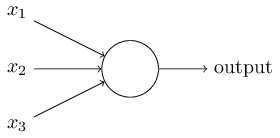
\includegraphics{Perceptron.png}
	\caption{A Single Perceptron}
\end{figure}

Frank Rosenblatt, the scientist who developed the perceptron in the 1950s and 1960s, devised a rule for computing the output from these neurons. Using what he called 'weights,' the importance of each input is assessed and expressed. Each input has a weight assigned to it, and the resultant output from these inputs - either a 1 or 0 - is dependent on whether or not some threshold value is less than or greater than the sum of the weights from all of the inputs to that particular perceptron. Therefore, if the weighted sum is less than or equal to the threshold value, the output is a 0. Otherwise, a 1\cite{4}. Both the threshold value and the input weights are real numbers. These can be tweaked to alter the decisions made by a neural network. 

\subsubsection{Sigmoid Neurons}

Sigmoid neurons are akin to perceptrons, however, they are modified in such a way that marginal alterations in their weights and bias cause only a small change to their output\cite{4}. This crucial difference is what affords a network consisting of sigmoid neurons the ability to learn.

The inputs to a sigmoid neuron also differ from those of perceptrons. Rather than being binary (1 or 0), these inputs are any number \textit{between} 1 and 0. %probably pointless italics
Much like with perceptrons, these sigmoid neuron inputs are weighted, with an overall bias included. These can be denoted \textit{b, $w_1$, $w_2$, ... $w_n$}
where \textit{b} represents the bias, and each \textit{w} is an input weight. This time however, the output is non-binary. To calculate it, we use 
\begin{eqnarray}
\sigma (w \cdot x+b)
\end{eqnarray}
where $\sigma$ is known as the sigmoid function, which is defined as:
\begin{eqnarray} 
\sigma(z) \equiv \frac{1}{1+e^{-z}}.
\end{eqnarray}
%*Incidentally, $\sigma$ is sometimes called the logistic function, and this new class of neurons called logistic neurons. It's useful to remember this terminology, since these terms are used by many people working with neural nets. However, we'll stick with the sigmoid terminology.*
In its full extended form, with \textit{x} being used to symbolise the inputs, the output of a sigmoid neuron is calculated as
\begin{eqnarray} 
\frac{1}{1+\exp(-\sum_j w_j x_j-b)}.
\end{eqnarray}

/////////////////////////////////////////////////////////////////////////////////\\
To understand the similarity to the perceptron model, suppose 
z
$\equiv w \cdot x + b$
is a large positive number. Then 
$e^{-z}
\approx 0$
and so 
$\sigma(z) \approx 1$
. In other words, when 
$z = w
\cdot x+b$
is large and positive, the output from the sigmoid neuron is approximately 1, just as it would have been for a perceptron. Suppose on the other hand that 
$z = w \cdot x+b$
is very negative. Then 
$e^{-z} \rightarrow \infty$
, and
$\sigma(z) \approx 0$
. So when 
$z = w \cdot x +b$
is very negative, the behaviour of a sigmoid neuron also closely approximates a perceptron. It's only when 
$w \cdot x+b$
is of modest size that there's much deviation from the perceptron model\cite{4}.

///////////////////////////////////////////////////////////////////////////////

\begin{figure}[h]
	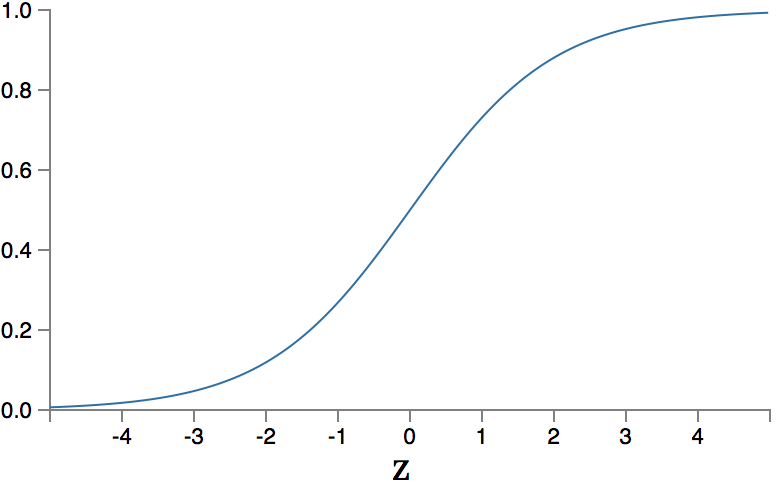
\includegraphics[width=\textwidth, height=5cm]{SigmoidFunction.png}
	\caption{Sigmoid Function}
\end{figure}

The shape of a plotted $\sigma$ function can be seen in Figure 2. 

///////////////////////////////////////////////////////////////////////////////
The smooth nature of $\sigma$ means that minor changes in the weights and bias - which are depicted as $\Delta w_j$ and $\Delta b_j$ respectively - will consequently create small changes to the output from the neuron. That change - $\Delta \mbox{output}$ - can be approximated with calculus:
\begin{eqnarray} 
\Delta \mbox{output} \approx \sum_j \frac{\partial \, \mbox{output}}{\partial w_j}
\Delta w_j + \frac{\partial \, \mbox{output}}{\partial b} \Delta b
\end{eqnarray}
The sum is over all of the weights, 
$w_j$, and 
$\partial \,
\mbox{output} / \partial w_j$
and
$\partial \, \mbox{output} /\partial
b$
denote partial derivatives of the output with respect to 
$w_j$
and 
\textit{b}, respectively.

As $\Delta \mbox{output}$ is a linear function of the changes
$\Delta w_j$ and $\Delta b_j$ in the weights and bias. This linearity makes it easy to choose small changes in the weights and biases to achieve any desired small change in the output. So while sigmoid neurons have much of the same qualitative behaviour as perceptrons, they make it much easier to figure out how changing the weights and biases will change the output.

///////////////////////////////////////////////////////////////////////////////\\
\subsection{Evolutionary Algorithms}
As the name might suggest, an evolutionary algorithm is one that evolves. It does so to encourage finding the most optimal solution to a problem. A vast amount of varying evolutionary algorithms exist, but at the core of them all is the same principal idea: "given a population of individuals the environmental pressure causes natural selection (survival of the fittest) and this causes a rise in the fitness of the population"\cite{5}.
\\
\subsection{NeuroEvolution for Augmenting Topologies (NEAT)}
"NEAT is a method for evolving speciated neural networks of arbitrary structures and sizes. NEAT leverages the evolution of structure to make neuroevolution more efficient"\cite{6}.
\\
\subsection{Summary}
.
\newpage
\section{Literature Review}
And so on for each of the chapters.  The template automatically starts new chapters on a new page.  The associated guidelines tell you what the available styles do and also how to structure a report.
There is a section break on this page that you should be careful NOT to delete otherwise the references and appendices will be numbered continuously with the rest of the document.

% another example section
\newpage
\section{Additional Information / Knowledge Required}
Experience with Linux and managing Virtual machines, networking.
So on and so forth...

\newpage
\begin{thebibliography}{9}

\bibitem{lamport94}
  Leslie Lamport,
  \emph{\LaTeX: A Document Preparation System}.
  Addison Wesley, Massachusetts,
  2nd Edition,
  1994.

\end{thebibliography}
%example of References. See https://en.wikibooks.org/wiki/LaTeX/Bibliography_Management
%might be good to use a separate document for these so your main work is not one really long text file. 

%you can crate this on a extra tex document just like the title or any other part of the document.
\newpage
\begin{appendices}
\section{Project Overview}
%insert IPO 

\Large{\textbf{Initial Project Overview}\\

\textbf{SOC10101 Honours Project (40 Credits)}}\\                                                      

\large{\textbf{Title of Project:}}

\normalsize{Evolution of Neural Network Controllers for Gameplay Behaviours} \\

\underline{\textbf{Overview of Project Content and Milestones}}

The idea is to implement a card game with four players. One of the players is the human, another is an AI agent that has no idea how to play the game, and the other two are hard-coded to know the rules and how to play. The intention is for said card game to be Switch, however this is subject to change if the rules are found to be too difficult for the scale of the project – in which case a simpler game will be substituted in.


The agent then learns how to play by trying to make moves based on neural networks. Initially this will be totally random but after the first generation of the algorithm cycle, it will be based on the chromosomes with the highest fitness, which should then begin to provide better results. These moves can be blocked if they are not legal. There'll be a scoring system for the agent that will be negatively affected by illegal moves and it will then use this to learn how to do better the next time it plays. The scoring system will also see the agent penalised for losing or not winning. This will be what our fitness is based on. 


It is worth noting that how successful you are in a game of Switch depends entirely on the hand you’re dealt, and how your opponents play the hands they are dealt. A lot of the game is about luck, and so negatively affecting the agent’s score should take this into account and deploy some leniency. 


The project will make use of the NeuroEvolution of Augmenting Topologies (NEAT) library and will most likely be coded in C++. It will use neural network controllers, co-evolving weights and topologies. \\

\pagebreak
\large{\textbf{The Main Deliverable(s):}}
\begin{itemize}
	\item A playable card game that incorporates an Artificial Intelligence agent that must learn how to play the game from scratch based on a score system that penalises the agent for illegal or costly decisions. 
	\item Experimental research into improving the performance (in terms of score) or speeding up the learning process of the agent. 
	\item A report into what positively or negatively affects the agent, and what causes the effects that it has including experiment results using charts and figures. Changes will be made by varying parameter settings of the evolutionary algorithm in a systematic way.
\end{itemize}

\large{\textbf{The Target Audience for the Deliverable(s):}}

Whilst the final product will be a playable game, it will really be aimed more at being experimental research into Artificial Intelligence techniques and, more specifically, evolving neural network controllers for playing games. Thus, the audience most likely to be interested in the project are those who also want to look into artificial intelligence agents. \\

\pagebreak
\large{\textbf{The Work to be Undertaken:}}
\begin{itemize}
	\item Design and build a game of Switch without the AI agent
	\item Thoroughly test the barebones game to ensure it works perfectly without bugs
	\item Research neural networks and evolutionary algorithms
	\item Implement the AI agent
	\item Experiment with a few different techniques and test how they perform in terms of improving or decreasing the agent’s intelligence/performance in game.
\end{itemize} 

\large{\textbf{Additional Information / Knowledge Required:}}

Neural networks and evolutionary algorithms\\

\large{\textbf{Information Sources that Provide a Context for the Project:}} %HATE how Project is on the next line here
\begin{itemize}
	\item Lubberts, \& Miikkulainen (2001). Co-Evolving a Go-Playing Neural Network.
	\item Stanley, Bryant, \& Miikkulainen (2005). Evolving Neural Network Agents in the NERO Video Game. IEEE Press.
	\item Thrun (1995). Learning to Play the Game of Chess. MIT Press. 
\end{itemize}

\large{\textbf{The Importance of the Project:}}

Exploring possibilities and limits of AI in games, particularly evolved controllers which do not have to be hard-coded.\\

\large{\textbf{The Key Challenge(s) to be Overcome:}}
\begin{itemize}
	\item Complete lack of knowledge and experience with Artificial Intelligence techniques
\end{itemize}


\begin{subappendices}
\subsection{Example sub appendices}
...
\end{subappendices}

\section{Second Formal Review Output}
Insert a copy of the project review form you were given at the end of the review by the second marker

\section{Diary Sheets (or other project management evidence)}
Insert diary sheets here together with any project management plan you have

\section{Appendix 4 and following}
insert content here and for each of the other appendices, the title may be just on a page by itself, the pages of the appendices are not numbered, unless an included document such as a user manual or design document is itself pager numbered.
\end{appendices}

\end{document}
